
% this file is called up by thesis.tex
% content in this file will be fed into the main document

%: ----------------------- introduction file header -----------------------
\chapter{Explainable Topic-based Associations}\label{ch:explainability}

\graphicspath{{explainability/figures/}}

% -------------------------------------------------------------
% -- Explainability
% -------------------------------------------------------------

As stated in Chapter \ref{ch:hypothesis}, one of our hypotheses aims to determine whether is possible to semantically relate texts from their most relevant topics (H1.2). In particular, our goal is to determine whether two documents can be related by identifying their most representative topics.

However, as seen in Section \ref{sec:topic-explainability}, interpreting how documents are related from their topic distributions is hard when using density-based measures. The same pair of documents may vary their distance from each other when using topic models with different dimensions to represent them, as shown in figure \ref{fig:topic_distances}. High dimensional models create more specific topics than models with fewer dimensions, and this topic specificity influences the way in which topic distributions are related. 

In order to better understand the relations derived from topic distributions, Section \ref{sec:topic-relations} compares scientific articles from their representations based on full-content, abstracts (i.e manual summaries), or summaries created automatically. Two types of metrics are considered: (i) \textit{internal-representativeness}, focused on describe the content, and \textit{external-representativeness}, focused on discover relations \citep{Badenes-Olmedo2017c}.    

In Section \ref{sec:topic-clustering}, once we know how the topics are used to represent and relate texts from their distributions, we propose a new topic-based annotation based only on the most representative topics and a new distance measure that takes advantage of these representations. The main goal is not only to relate texts through their most relevant topics, but also to facilitate their interpretation. 


\section{Topic-based Relations}
\label{sec:topic-relations}

This section studies the ability of topic distributions to capture the representativeness of a text through the relations that can be derived from it. In particular, it examines the performance offered by topic-based representations to describe scientific articles from their full-texts compared to representations based only on summaries (e.g. \textit{abstract}). The main objective is to analyze distances based on topic distributions on the one hand, and on the other hand to identify strengths and weaknesses when using \textit{abstracts} to compare scientific articles. Two novel measures are proposed based on the capability of the summary to substitute the original paper: (1) \textit{internal-representativeness}, which evaluates how well the summary represents the original full-text and (2) \textit{external-representativeness}, which evaluates the summary according to how the summary is able to produce a  set of related texts that are similar to what the original full-text has triggered.

Recent studies \citep{Westergaard2017, Sciences2016} have shown that text mining of full research articles give consistently better results than using only their corresponding abstracts. Given the size limitations and concise nature of abstracts, they often omit descriptions or results that are considered to be less relevant but still are important in certain Information Retrieval (IR) tasks. Thus, when other researchers cite a particular paper, 20\% of the keywords that they mention are not present in the abstract \citep{Divoli2012}.

\begin{figure}[!htbp]
\centering
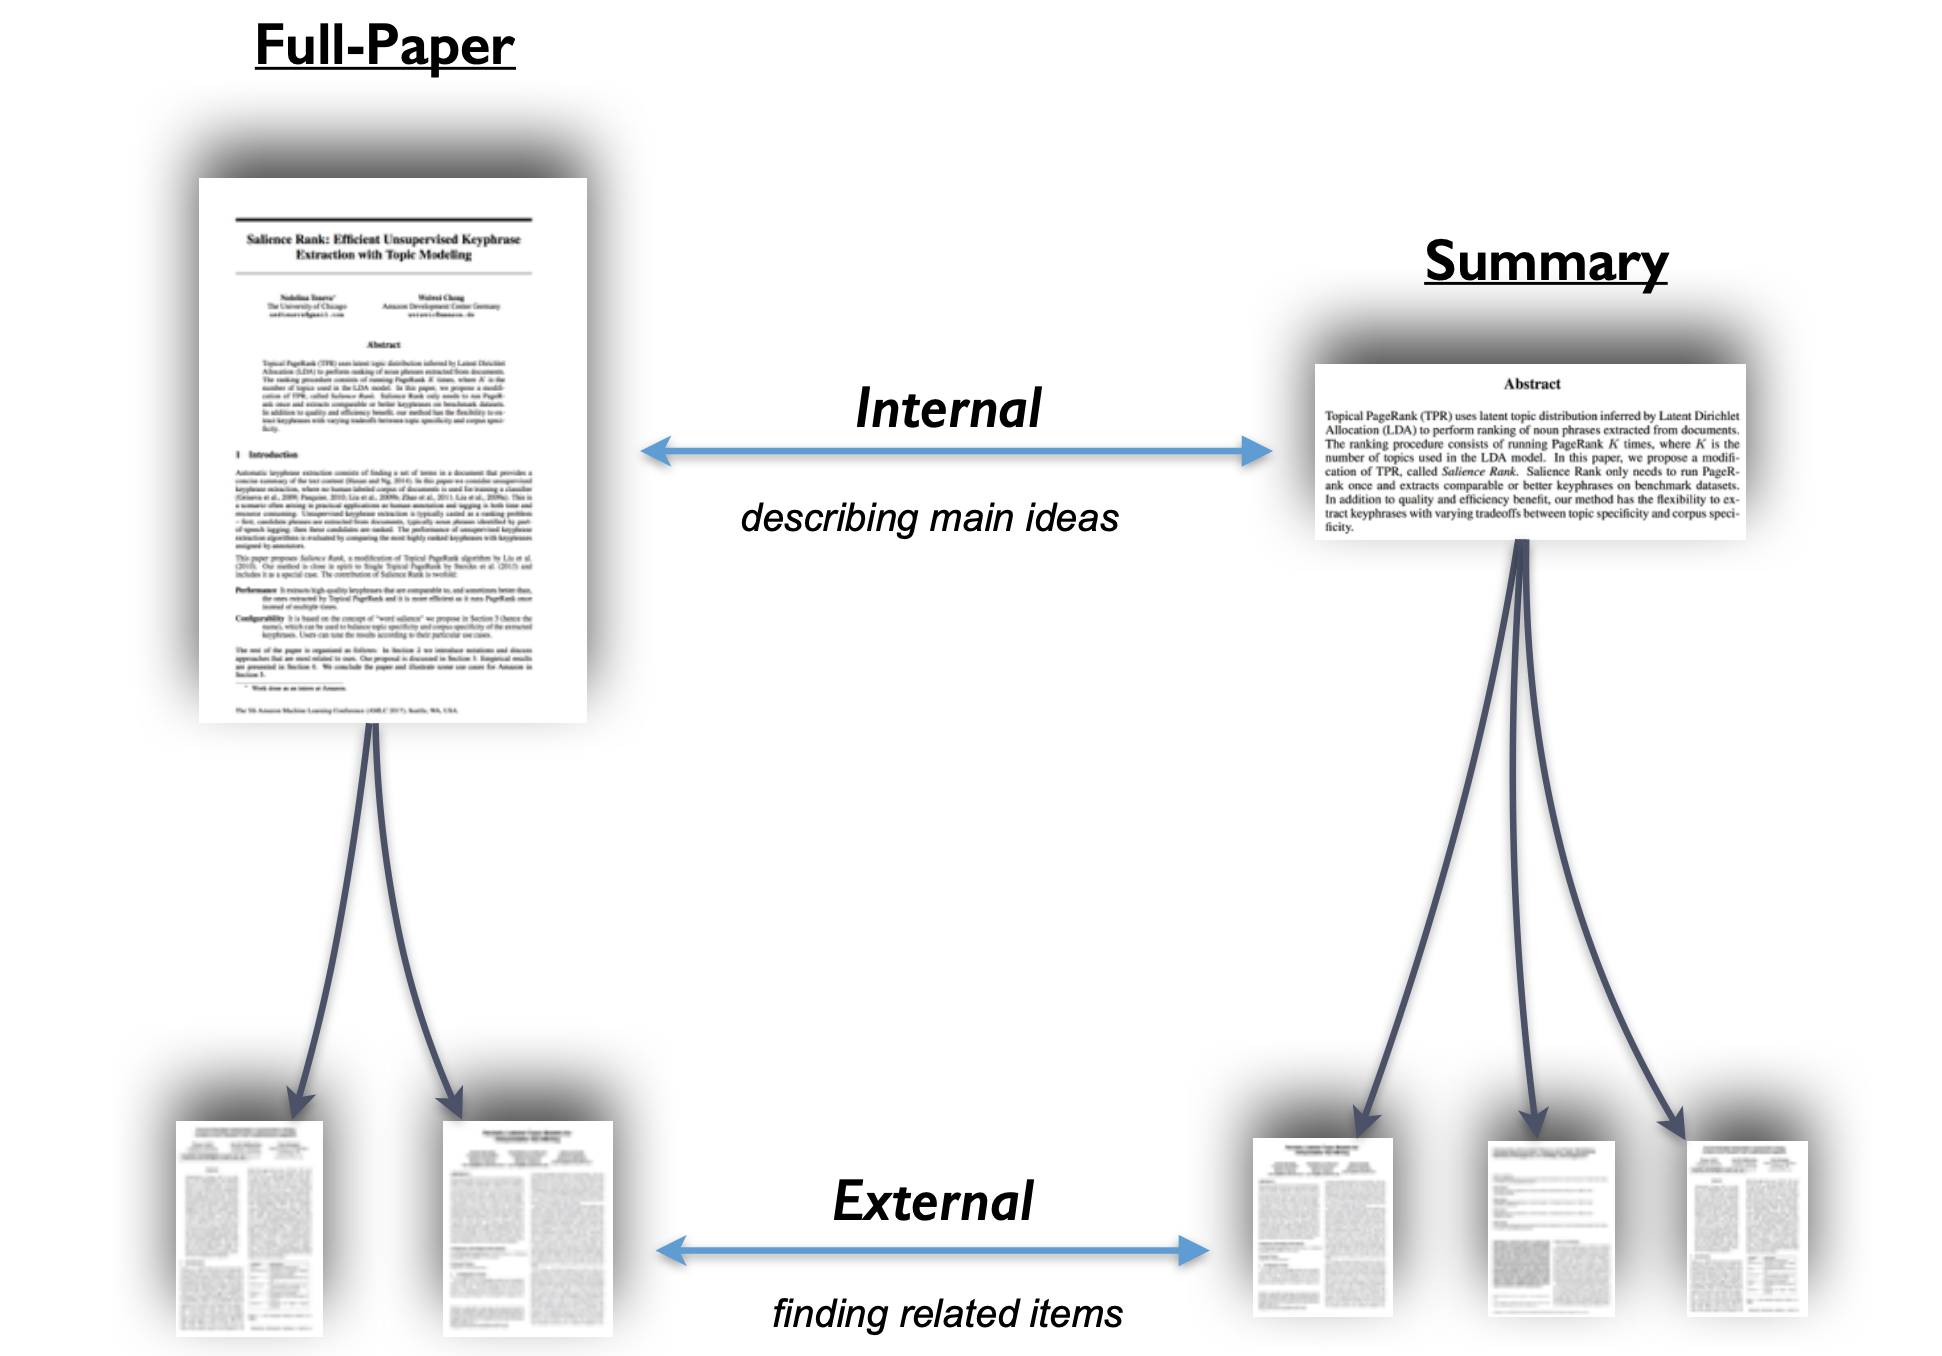
\includegraphics[scale=0.24]{internal-external.png}
\caption{Internal and External Representativeness. }
\label{fig:dimensions}
\end{figure}


An analysis about the \textit{representativeness} of research article summaries based on topic distributions is presented, considering those based exclusively on abstracts and those based on their discursive structure (\textit{approach}, \textit{challenge}, \textit{background}, \textit{outcomes} and \textit{future work})\citep{SimoneTeufel2010}. The \textit{representativeness} of a summary with respect to the original full-text is assumed as the degree of relation with the original one (\textit{internal-representativeness}), along with the capacity of mimicking the full text when finding related items (\textit{external-representativeness}). In order to quantify this notions of internal-external representativeness, a probabilistic topic model is trained to have a vectorial representation of each text retrieved from a paper: full content-based and summary-based. The vectorial representations of full-papers is used to measure the distance between them and those derived from abstract or summaries (\textit{internal-representativeness}), and also to find similar documents (\textit{external- representativeness}) based on the distance between their vectorial representations. An upper distance threshold is specified to filter less similar pairs and compose a set of related papers for each paper. Then, a comparison in terms of \textit{precision} and \textit{recall} is performed between sets obtained by only using the vectorial representation of full-papers, against sets produced by using other kind of summaries.

\subsection{Summaries based on Rhetorical Discourse parts}
\label{sec:annotator}
Some approaches have been proposed to summarize scientific articles \citep{Cohan2015} taking advantage of the citation context and the document discourse model. We have used the scientific discourse annotator proposed by \citep{Ronzano2015} to automatically create summaries from scientific articles by classifying each sentence as belonging to one of the following scientific discourse categories: \textit{approach}, \textit{challenge},  \textit{background}, \textit{outcomes} and \textit{future work}. These categories were identified from the schemata proposed by \citep{Teufel2009} with the original purpose of characterizing the content of Computer Graphics papers. The annotator is based on a Support Vector Machine classifier that combines both lexical and syntactic features to model each sentence in a paper. This tool\footnote{http://backingdata.org/dri/library/} was integrated in our \textit{librAIry} framework through the \textit{Rhetoric Module}\footnote{https://github.com/librairy/annotator-rhetoric} to automatically annotate research papers with their rhetorical content.

\subsection{Topic Distributions}
\label{sec:topicmodel}
A representational model is required not only to measure distances between text fragments but, more importantly, to help to understand the differences in their content. As seen in Section \ref{sec:topic-explainability}, topic models are widely used to uncover the latent semantic structure from text corpora. In particular, Probabilistic Topic Models represent documents as a mixture of topics, where topics are probability distributions over words. Latent Dirichlet Allocation (LDA)\citep{Blei2003} is the simplest \textit{generative} topic model that makes it possible to characterize documents not previously used during the training task. This is a key feature for our evaluations because, although the model used for the experiments will be trained from the full-content of papers, it will be also used to describe the texts summaries.

Thus, we have used a LDA model to describe the inherent topic distribution of papers in the corpus. Some hyper-parameters need to be estimated: the \textit{number of topics (k)}, the  concentration parameter ($\alpha$) for the prior placed on documents' distributions over topics and the concentration parameter ($\beta$) for the prior placed on topics’ distributions over terms. Since the target of this experiment is not to evaluate the quality of the representational model, but to compare their topic distributions, we accepted as valid values those widely used in the literature: $\alpha=0.1$, $\beta=0.1$ , and $k=2*\sqrt{n/2}=44$ where $n$ is the size of the corpus.

\subsection{Similarity Measure}
Feature vectors in Topic Models are topic distributions expressed as vectors of probabilities. Hence we opt for \textit{Jensen-Shannon divergence} (JSD)\citep{Lin1991} instead of the commonly used \textit{Kullback-Liebler divergence} (KLD). The reason for this is that KLD (1) is not defined when a topic distribution is zero and (2) is not symmetric, what does not fit well with semantic similarity measures which in general are symmetric \citep{Rus2013}. JSD considers the average of the distributions as follows :

\begin{equation}
JSD(p,q) = \sum\limits_{i=1}^T p_{i}*\log \frac{2*p_{i}}{p_{i}+q_{i}}  +  \sum\limits_{i=1}^T q_{i}*\log \frac{2*q_{i}}{q_{i}+p_{i}}
\label{eq:jsd}
\end{equation}
where  $T$ is the number of topics and $p,q$ are the topics distributions.

And the \textit{similarity measure} used in our analysis is based on the JSD transformed into a similarity measure as follows \citep{Dagan1998} :

\begin{equation}
similarity(D_i , D_j) = 10^{- JSD(p,q)}
\label{eq:simcontent}
\end{equation}
where  $D_i,D_j$ are the documents and $p,q$ the topics distributions of each of them.

\subsection{Experiments}
\label{sec:topic-relevance-experiments}

The corpus used in the experiments was created by combining journals in different scientific domains such as \textit{Advances in Space Research}, \textit{Procedia Chemistry}, \textit{Journal of Pharmaceutical Analysis} and \textit{Journal of Web Semantics}. In total 1,000 papers were added, 250 from each journal. Both the abstract and the \textit{full-content} of these documents were directly retrieved from the Elsevier API \footnote{https://dev.elsevier.com} by using our \textit{Harvester module} \footnote{https://github.com/librairy/harvester-elsevier}. The code used to perform the analysis along with the results obtained are available in GitHub\footnote{https://github.com/librairy/study-semantic-similarity}.

Since the annotation process to automatically discovers the rhetorical parts of a research paper (Section ~\ref{sec:annotator}) is sensitive to the structure of the phrases that are used when writing the text, only $20\%$ of papers in the corpus could be fully annotated with all the fragments considered. In fact, these categories are not present in the same proportion in the corpus: \textit{approach} ($90\%$), \textit{background} ($78\%$), \textit{outcome} ($73\%$), \textit{challenge} ($57\%$) and \textit{future work} ($21\%$)

\subsubsection{Internal Representativeness}

The \textit{internal-representativeness} of a summary measures the similarity of this summary against the original full-text research paper. This similarity is based on the JSD between the topic distribution of each of them. 

\begin{figure}[!htb]\centering
   \begin{minipage}{0.49\textwidth}
     \frame{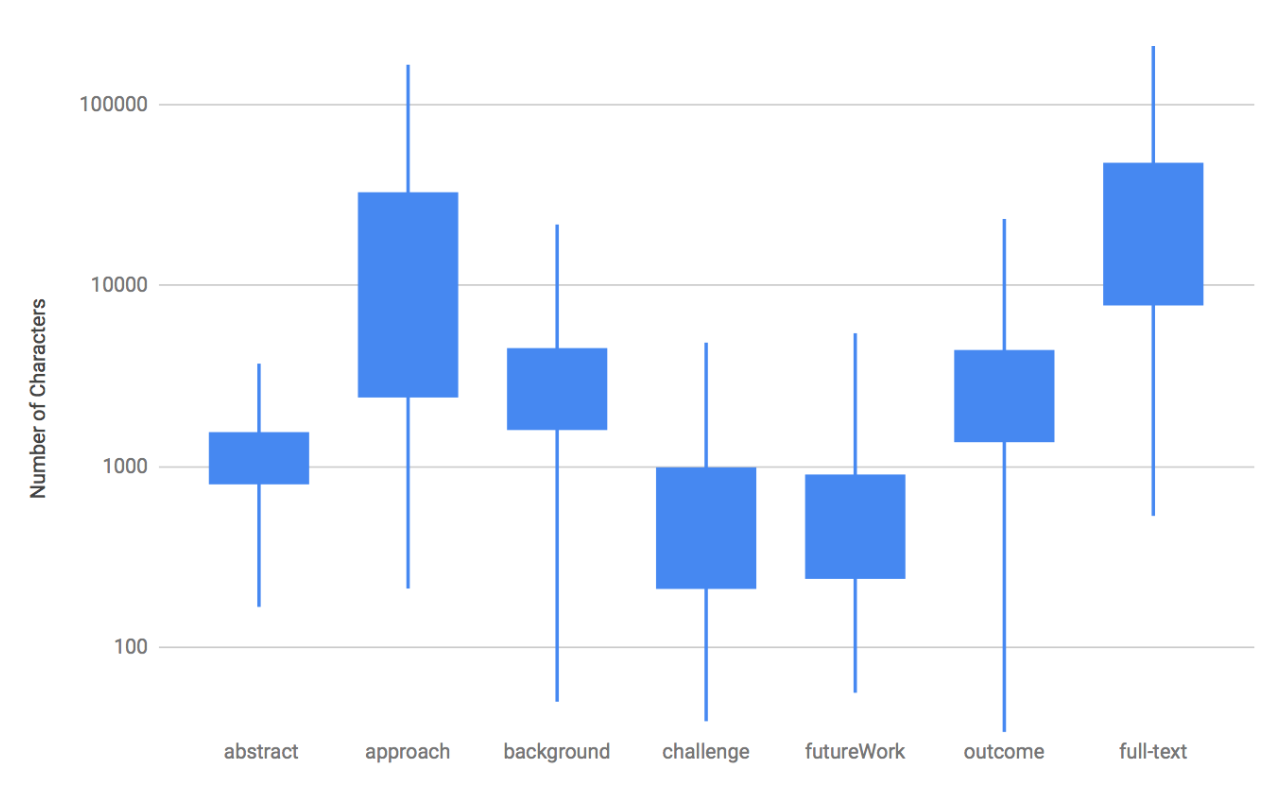
\includegraphics[width=\linewidth]{size.png}}
     \caption{length of summaries}\label{fig:size}
   \end{minipage}
   \begin {minipage}[c]{0.49\textwidth}
     \frame{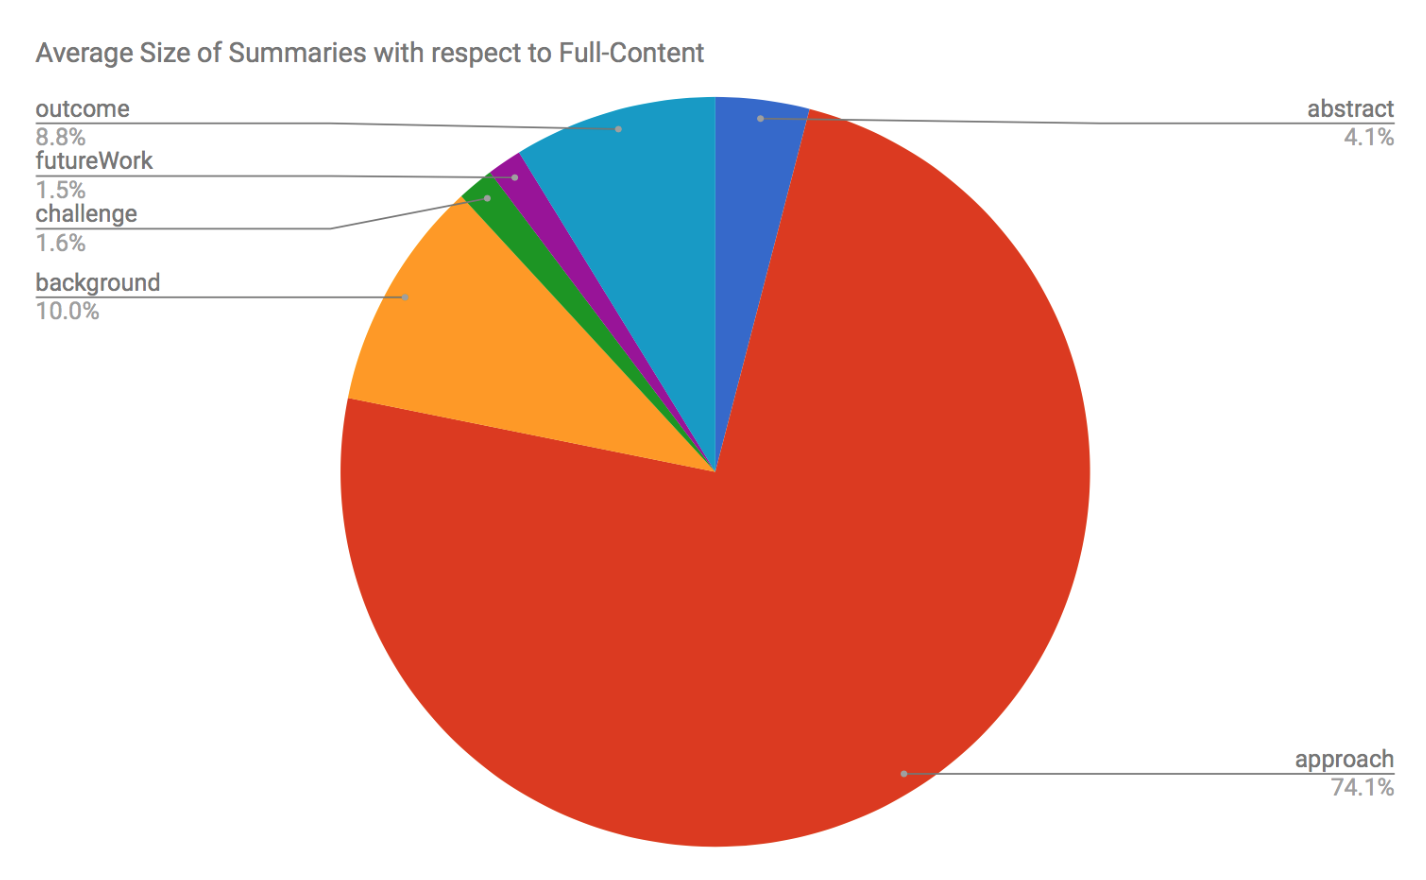
\includegraphics[width=\linewidth]{relativeSize.png}}
     \caption{relevance of text parts}\label{fig:relativeSize}
   \end{minipage}
\end{figure}

Since LDA considers documents as \textit{bag-of-words}, the text length (e.g. full-content or summaries) affects the accuracy of the topic distributions inferred by the topic model described in Section~\ref{sec:topicmodel}. The occurrences of words in short texts are less discriminative than in long texts where the model has more word counts to know how words are related \citep{Hong2010}. In view of the above, the \textit{approach}, the \textit{background} and the \textit{outcome} content of a paper generate more accurate topic distributions than those created from other approaches such as the abstract. Also, the relative presence of each of them in a paper (figure~\ref{fig:relativeSize}) shows an unexpected result when compared to the IMRaD format \citep{Nair2014}. This style proposes to distribute the content of an abstract, and by extension the full-paper, as follows: \textit{Introduction}(25\%), \textit{Methods}(25\%), \textit{Results}(35\%) and \textit{Discussion}(15\%). However, the results (figure~\ref{fig:relativeSize}) show that \textit{Method} section (\textit{approach} content) is more extensive than \textit{Results} section (\textit{outcome} content) in our corpus.

All pairwise similarities between full-papers, abstracts and rhetorical-based summaries are calculated to measure the \textbf{\textit{internal-representativeness}} of a summary with respect to the original text, i.e. the topic-based similarity value (equation~\ref{eq:simcontent}) between the probability distributions of the full-text and each of the summaries. Results (table~\ref{tab:irepresentativeness}) suggest than summaries created from the \textit{approach} content are more representative than others, i.e. the distribution of topics describing the text created from the \textit{approach} content is the most similar to the one corresponding to the full-content of the paper.

\begin{table}[!htb]
    \centering
        \begin{tabular}{l*{6}{c}r}\hline
                        & Min & Lower Quartile & Upper Quartile & Max & Dev  & Median \\
          \hline
          abstract & 0.0489 & 0.9109 & 0.9840 & 1.0000 & 0.1443 & 0.9741 \\
          \textbf{approach} & \textbf{0.0499} & \textbf{0.9969} & \textbf{1.0000} & \textbf{1.0000} & \textbf{0.0872} & \textbf{0.9998} \\
          background & 0.0463 & 0.8967 & 0.9937 & 0.9988 & 0.2037 & 0.9822 \\
          challenge & 0.0426 & 0.7503 & 0.9517 & 0.9940 & 0.2224 & 0.8829 \\
          futureWork & 0.0000 & 0.6003 & 0.9435 & 0.9948 & 0.2842 & 0.8814 \\
          outcome & 0.0485 & 0.9267 & 0.9925 & 0.9990 & 0.1721 & 0.9835 \\
        \end{tabular}
    \caption{Internal-Representativeness}\label{tab:irepresentativeness}
\end{table}

\subsubsection{External-Representativeness}  

The \textit{external-representativeness} metric tries to measure how different is the set of related documents obtained from summaries with respect to those derived from the original full-text. In terms of \textit{precision}, \textit{recall} and \textit{f-measure}, a comparison has been performed to analyze the behavior of the summaries when trying to discover related content compared to use the full-text of the article.

By using the same topic model previously created, similarities among all pairs of documents were also calculated according to equation~\ref{eq:simcontent}. Then, a minimum score or similarity threshold is required to define when a pair of papers are related. Each threshold is used to create a gold-standard which relates articles to others based on their similarity values. In order to discover that lower bound of similarity, a study about trends in the similarity scores (fig~\ref{fig:similarities}) as well as distributions of topics in the corpus (fig~\ref{fig:articleTopics}) was performed. We can see that topics are not equally balanced across papers. This fact generates separated groups of strongly related papers. We think this phenomena is due to our usage of a corpus created from journals where different domains are equally balanced. Then, we considered a similarity score equals to $0.99$ (fig ~\ref{fig:similarities}) as the threshold from which strong relations appear. However, to cover different interpretations of similarity, from those based on sharing general ideas or themes to those that imply to share a more specific content, the following list of thresholds was considered in the experiments: 0.5, 0.6, 0.7, 0.8, 0.9, 0.95 and 0.99.

\begin{figure}[!htb]\centering
   \begin{minipage}{0.49\textwidth}
     \frame{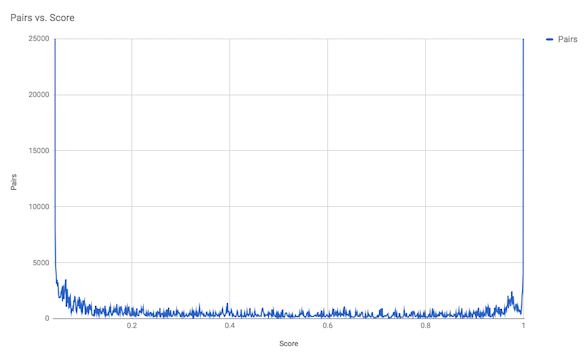
\includegraphics[width=\linewidth]{similarities.png}}
     \caption{number of pairwises by similarity score (rounded up to two decimals)}\label{fig:similarities}
   \end{minipage}
   \begin {minipage}[c]{0.49\textwidth}
     \frame{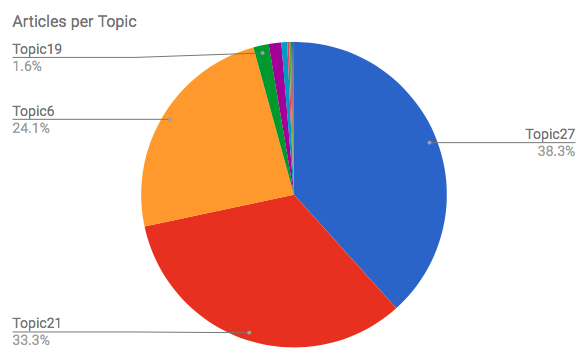
\includegraphics[width=\linewidth]{articlesTopic.png}}
     \caption{topics per article with value above 0.5}\label{fig:articleTopics}
   \end{minipage}
\end{figure}

For each similarity threshold, a gold-standard was created based on considering as related those papers with a similarity value upper than the selected threshold. Results ( figure ~\ref{fig:precision}) comparing the related papers inferred from the full-content with those inferred from the partial-content representation (i.e. abstract or rhetorical parts) suggest that strongly related papers are mainly discovered by using the summary created from the \textit{approach} section. The reason for this may be based on the average size of this type of summaries or the particular content included in this part of a paper. While other summaries include more general-domain words, the \textit{approach} content includes more specific words that describe the method or the final objective of the paper. So, for higher similarity thresholds, i.e. for strongly related papers, the recommendations discovered by using the \textit{approach} are more precise than those discovered by using the abstract.

\begin{figure}[!htb]\centering
   \begin{minipage}{0.49\textwidth}
     \frame{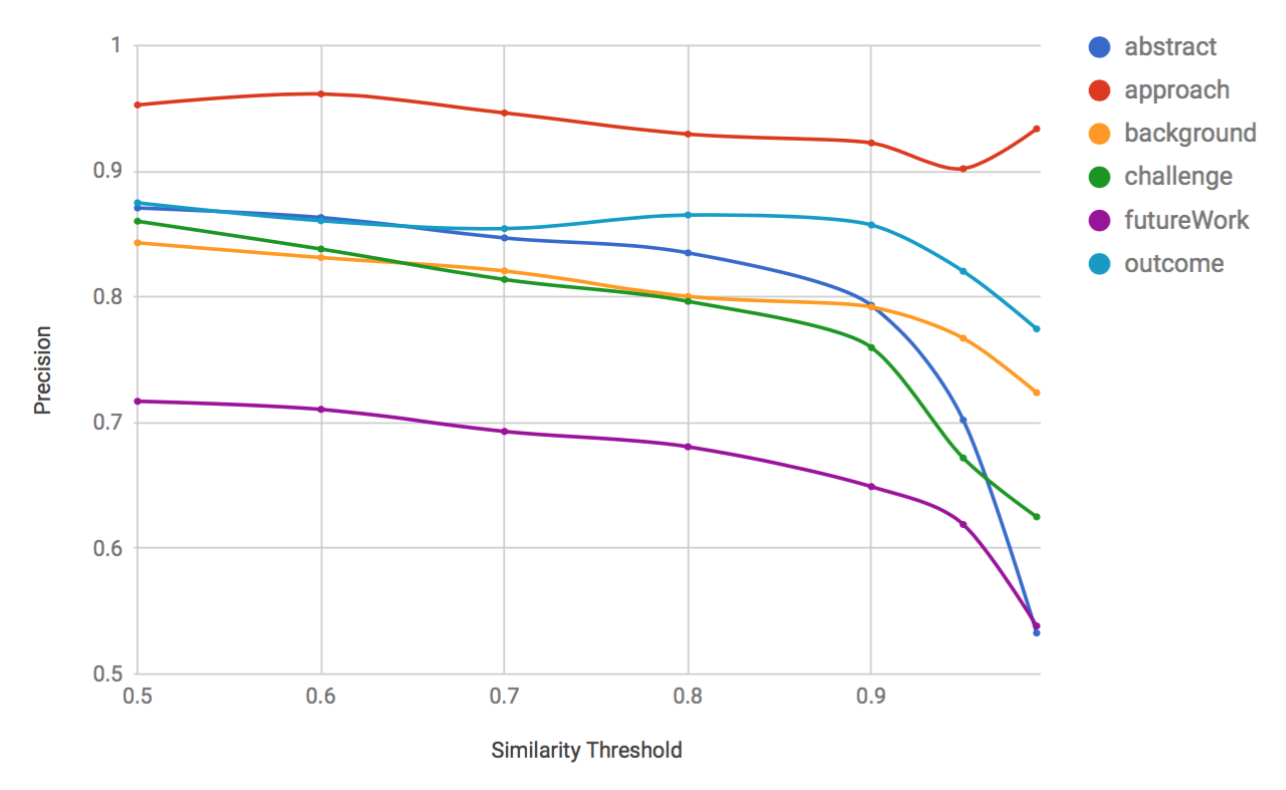
\includegraphics[width=\linewidth]{precision.png}}
     \caption{P at different similarity thresholds}\label{fig:precision}
   \end{minipage}
   \begin {minipage}[c]{0.49\textwidth}
     \frame{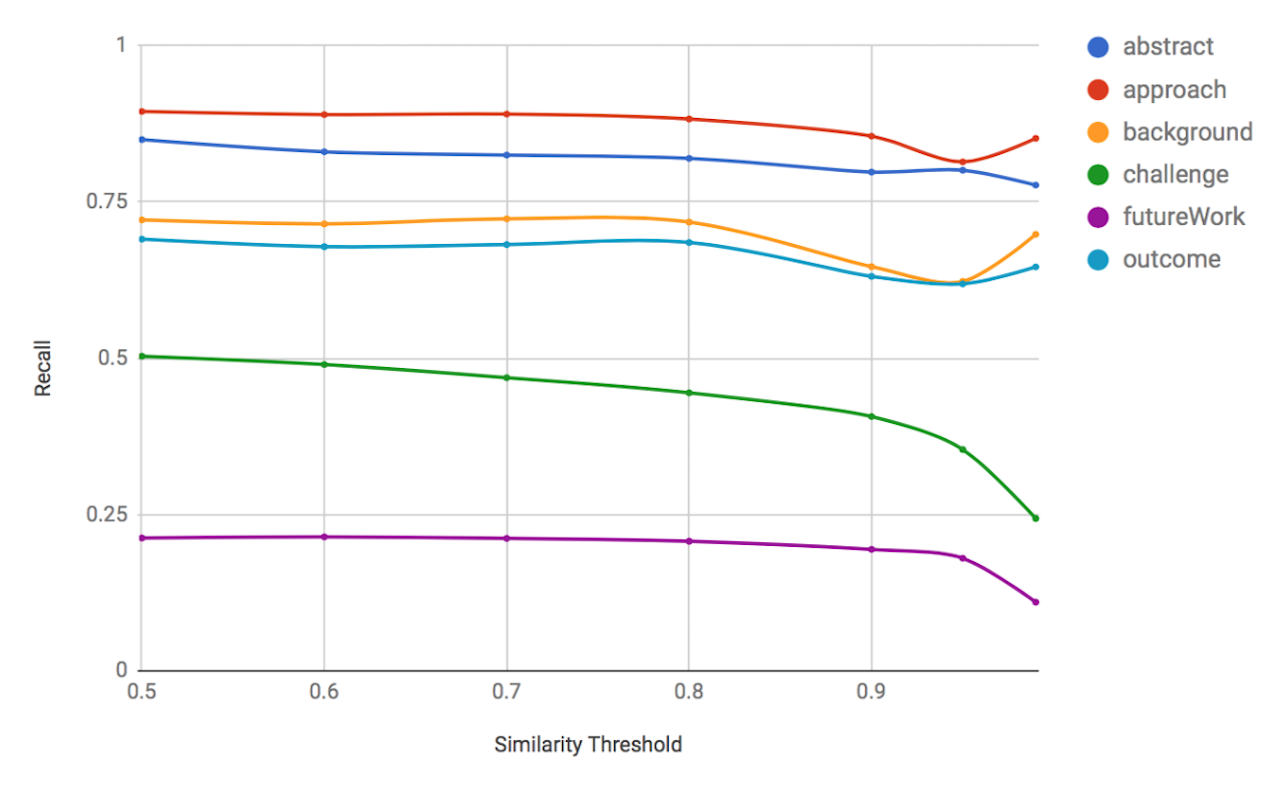
\includegraphics[width=\linewidth]{recall.png}}
     \caption{R at different similarity thresholds}\label{fig:recall}
   \end{minipage}
\end{figure}

In terms of \textit{recall} (figure ~\ref{fig:recall}), the upward trend followed by the \textit{approach}, the \textit{outcome} and the \textit{background} content remarks the assumption of summaries containing key words allow to discover more similar papers than others. Moreover, since \textit{recall} overlooks false-negatives classifications, it suggests that these parts of a research paper share more words than others with strongly related papers but they may also present commonalities with highly related papers, except in case of \textit{approach} which still exhibits higher \textit{precision}.

As expected, only summaries created from the \textit{approach}, the \textit{outcome} and the \textit{background} content maintain high accuracy values (fig~\ref{fig:fmeasure}) even for high similarity thresholds. Along with the results showed in figure~\ref{fig:stdeviation}, where the same three rhetorical classes present the lowest standard deviation over the \textit{f-measure}, they can be considered as the most robust summaries containing the ideas that better characterize the paper compared to others.

\begin{figure}[!htb]\centering
   \begin{minipage}{0.49\textwidth}
     \frame{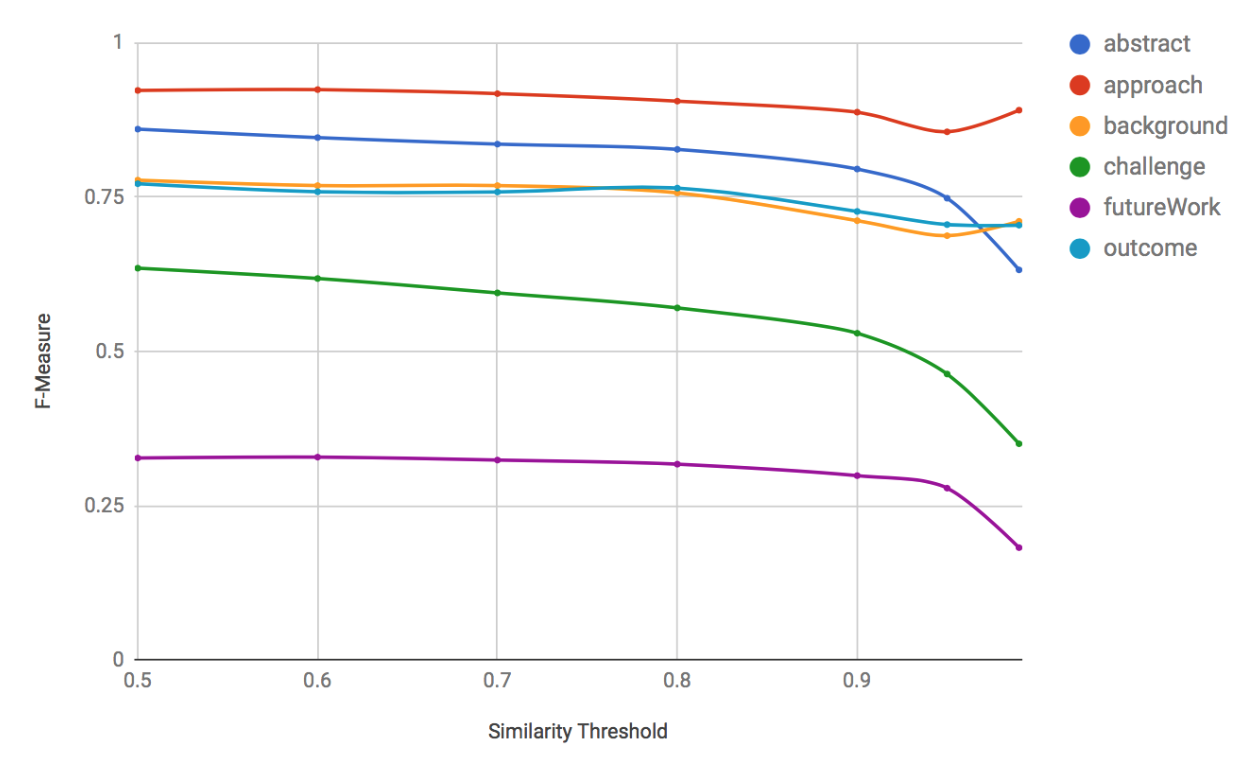
\includegraphics[width=\linewidth]{fmeasure.png}}
     \caption{f-measure performance}\label{fig:fmeasure}
   \end{minipage}
   \begin {minipage}[c]{0.49\textwidth}
     \frame{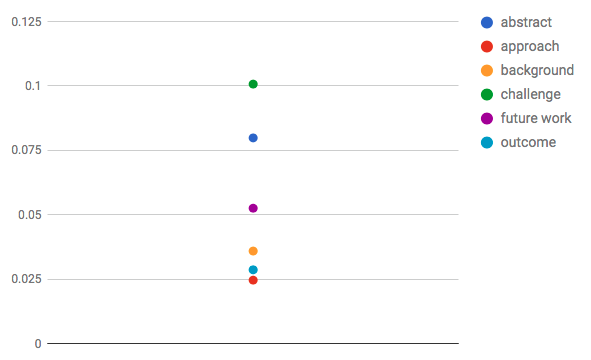
\includegraphics[width=\linewidth]{stdeviation.png}}
     \caption{f-measure deviation}\label{fig:stdeviation}
   \end{minipage}
\end{figure}

\subsection{Summary}
Topic-based similarities have been studied among scientific documents based on their abstract sections with respect to summaries corresponding to their scientific discourse categories. For this purpose, two novel measures have been proposed: (1) \textit{internal-representativeness} and (2) \textit{external-representativeness}.

Results show that summaries created from the \textit{approach}, \textit{outcome} or \textit{background} content of a paper describe more accurately its full-content in terms of overall ideas and related documents than abstracts. Although those summaries are more extensive in number of characters than other with similar \textit{precision} such as the abstract content, they have proven to be particularly helpful  discovering strongly related papers, i.e. papers with a similarity value close to 1.0.


\section{Topic-based Clustering}
\label{sec:topic-clustering}


\section{Summary}

In Section \ref{sec:topic-relations}, we have analyzed the representativeness of topics to describe texts. In the particular case of scientific articles, it is concluded that the abstracts are not sufficiently representative to describe, by means of topics, the content of a paper. This behavior suggests that texts with greater vocabulary that emphasize key terms through repetition, favor topic-based representation.

Taking into account the relevance of topics to describe texts, we analyze in Section {\ref{sec:topic-clustering}} the behavior of topic distributions to calculate distances between documents using topic models with different dimensions. By using clustering techniques at the topic level, the most representative topics of a topic distribution are identified regardless of the number of dimensions that the model has. A topic-based representation is then proposed that covers the third research objective of this thesis (R03, \textit{define annotations based on topics that enable a semantic-aware exploration of the knowledge inside a corpus}). 

A new distance metric is also proposed that takes advantage of such representation to compare documents. Its performance is analyzed by automatically clustering the JRC-Acquis corpus according to EUROVOC categories. Tables XX and XY show results with high precision and recall in unsupervised classification tasks. This new way of relating documents from their most representative topics covers the fourth research objective of this thesis (R04, \textit{define a metric based on topic annotations that compares documents and facilitates their interpretation}). 

In order to perform the experiments, both the representation based on the most relevant topics and the distance metric based on these representations have been implemented in \textit{librAIry}. This partially covers the third and fourth technical objectives (T03, \textit{integrate the annotation method base on topic hierarchies into the topic model service}) (T04, \textit{create a system capable of finding similar document automatically}).